\section{Auswertung}

Im ersten Versuchsteil wurde die longitudinale Relaxationszeit $T_1$ gemessen. 
Die Werte der Messung sind in Tab. \ref{tab:t1} aufgetragen. 
In Abb. \ref{abb:t1} sind die Daten dargestellt worden und nach Formel \eqref{eq:t1} wurde ein Fit an die Daten durchgeführt.

\begin{table} \caption{Die variierenden Pulsabstände $\tau$ sind hier gegen die zugehörigen Amplituden, die am Oszilloskop gemessen wurden, aufgetragen.}
    \label{tab:t1}
    \centering
    \sisetup{round-mode = places, round-integer-to-decimal=true}
    \begin{tabular}{S[] S[] | S[] S[]}
        \toprule
        {$\tau / \si{\second}$} & {Amplitude / $\si{\volt}$} & {$\tau / \si{\second}$} & {Amplitude / $\si{\volt}$} \\
        \midrule
        1e-4&  -1.41    &        0.9  &  -0.66    \\
        1e-2&  -1.38    &        1.0  &  -0.607   \\
        0.05&  -1.34    &        1.2  &  -0.505   \\
        0.1 &  -1.27    &        1.4  &  -0.405   \\
        0.2 &  -1.19    &        1.6  &  -0.302   \\
        0.3 &  -1.11    &        1.8  &  -0.127   \\
        0.4 &  -1.03    &        1.85 &  -0.108   \\
        0.5 &  -0.952   &        1.9  &  -0.098   \\
        0.6 &  -0.877   &        1.95 &  -0.079   \\
        0.7 &  -0.8     &        2.1  &   0.044   \\
        0.8 &  -0.73    &        2.2  &   0.160 \\
            &           &        2.3  &  0.212  \\
        \bottomrule
    \end{tabular}
\end{table}

\begin{figure}
    \centering
    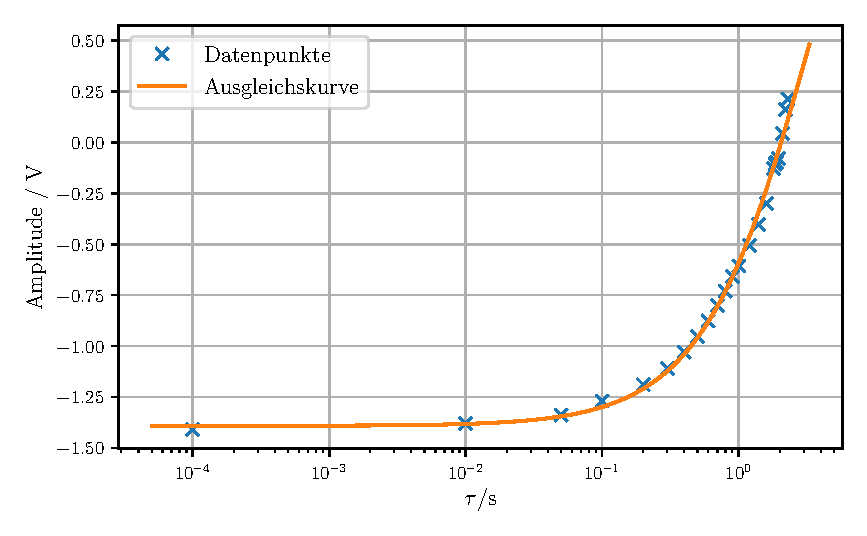
\includegraphics[width=\textwidth]{plots/T1.pdf}
    \caption{Die Pulsabstände $\tau$ sind gegen die zugehörigen Amplituden aufgetragen. Die Zeit-Achse ist logarithmiert worden.}
    \label{abb:t1}
\end{figure}

Die Parameter, die sich aus dem Fit ergeben sind 
\begin{align*}
    M_0 &= \SI{1.39(2)}{\volt} \\
    T_1 &= \SI{2.96(4)}{\second} \\.
\end{align*}
Im nächsten Versuchsteil wurden die transversale Relaxationszeit $T_2$ bestimmt. 
Dafür wurde die Meiboom-Gill-Methode verwendet. An die Maxima eines mit dem Oszilloskop aufgezeichneten Ereignisses wurde ein Fit mit der Funktion mit der Funktion \eqref{eq:t2} durchgeführt. Diese Daten und der Fit sind in Abb. \ref{abb:t2} zu sehen. 

\begin{figure}
    \centering
    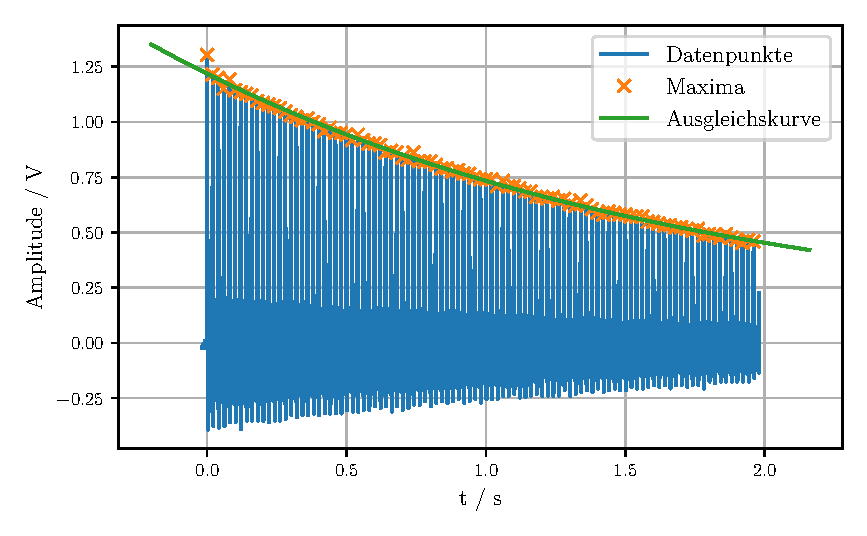
\includegraphics[width=\textwidth]{plots/T2.pdf}
    \caption{Ein Ereignis der Meiboom-Gill-Methode wurde gemessen und ein Fit an die Maxima wurde durchgeführt. Die Maxima der Daten sind hier hervorgehoben worden.}
    \label{abb:t2}
\end{figure}

Die Parameter, die sich daraus ergeben haben, sind 
\begin{align*}
    M_0 &= \SI{1.15(3)}{\volt} \\
    M_1 &= \SI{65.73(3227)}{\milli\volt} \\
    T_2 &= \SI{1.83(8)}{\second} \\.
\end{align*}

Die letzte zu messende Größe ist die Diffusionskonstante $D$. Neben den Echohöhen muss dafür der Gradient $G$ mithilfe einer Fourier-Transformation gemessen werden. 
Das gemessene Spektrum ist in Abb. \ref{abb:spektrum} zu sehen. Die Abbildung zeigt das Otto-Hahn-Verfahren.
\begin{figure}
    \centering
    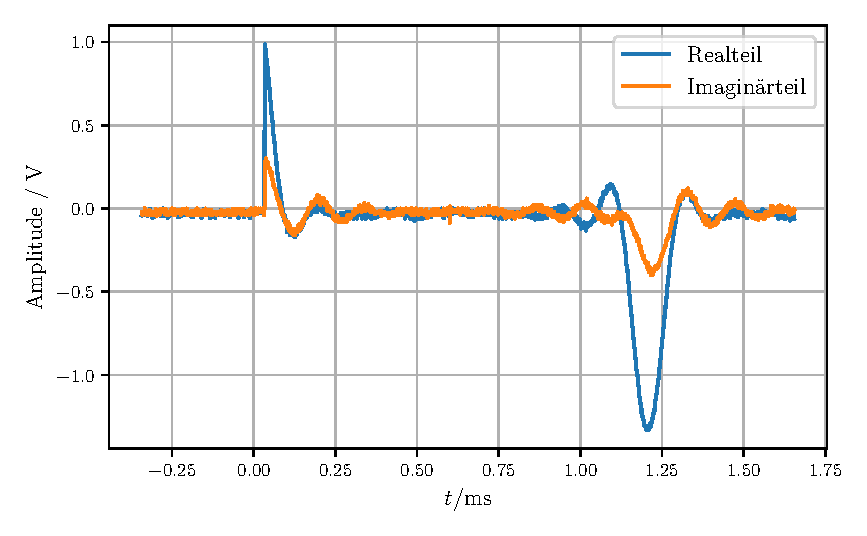
\includegraphics[width=0.8\textwidth]{plots/spektrum.pdf}
    \caption{Hier ist das Spektrum des Otto-Hahn-Verfahrens bei einer kleinen Pulslänge gemessen worden. Die Daten werden benutzt um mittels einer Fourier-Transformation die letzten fehlenden Daten zur Bestimmung der Gradientenstärke zu ermitteln.}
    \label{abb:spektrum}
\end{figure}

Nach der Fourier-Transformation ergibt sich die Abb. \ref{abb:fourier}.
\begin{figure}
    \centering
    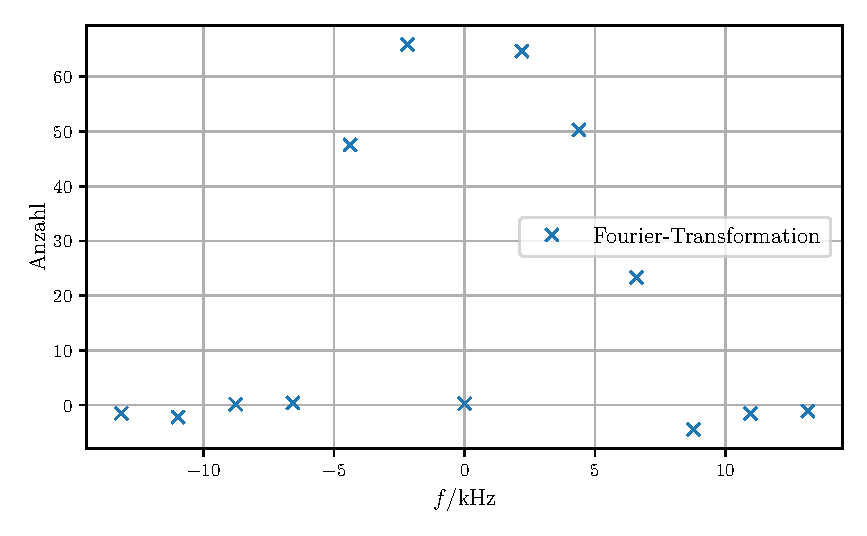
\includegraphics[width=0.8\textwidth]{plots/echo_gradient.pdf}
    \caption{Die Fourier-Transformierte der Daten in Abb. \ref{abb:spektrum}. Aus den Nullstellen lässt sich der Gradient bestimmen.}
    \label{abb:fourier}
\end{figure}
Der Abstand der Nullstellen auf der Frequenzachse beträgt demnach 
\begin{align*}
d_f = \SI{15.35}{\kilo\hertz}.
\end{align*} 
Die Gradientenstärke lässt sich mit den bekannten Größen der Probenform
\begin{align*}
    \gamma &= \SI{267.5e6}{\per\second\per\tesla} \\
    d_\text{Probe} &= \SI{4.4}{\milli\metre} \\ 
    \end{align*} 
und dem Faktor $d_f$ berechnen.
Der Faktor $\gamma$ ist dabei das gyromagnetische Verhältnis für Protonen (\cite{scipy}, der CODATA 2018 Wert), $d_\text{Probe}$ ist der Innendurchmesser der Probe.
Der Zusammenhang zwischen den Größen und der Gradientenstärke $G$ ist
\begin{equation*}
G = 2 \pi \frac{d_f}{d_\text{Probe} \gamma}.
\end{equation*}
Somit ergibt sich ein Wert von 
\begin{equation*}
G = \SI{0.0819}{\tesla\per\metre}.
\end{equation*}



Das letzte was zur Bestimmung der Diffusionskonstante benötigt wird sind die gemessenen Echohöhen. In Tab. \ref{tab:t2} sind die Pulslängen gegen die Echohöhen aufgetragen. Die Daten sind in Abb. \ref{abb:echo} mit einem Fit der Funktion \eqref{eq:echo} dargestellt. 

\begin{table} \caption{Die variierenden Pulsabstände $\tau$ sind hier gegen die zugehörigen Amplituden, die am Oszilloskop gemessen werden, aufgetragen.}
    \label{tab:t2}
    \centering
    \sisetup{round-mode = places, round-integer-to-decimal=true}
    \begin{tabular}{S[] S[] | S[] S[]}
        \toprule
        {$\tau / \si{\second}$} & {Amplitude $/ \si{\volt}$} & {$\tau^3 / \si{\micro\second}$} & {$\ln\left(M(\tau)\right) - 2\tau/T_2$} \\
        \midrule
        1e-4  &  1.51   &  1.000000000000000167e-06 & 4.120005768950588121e-01 \\
        1e-3  &  1.5    &  1.000000000000000021e-03 & 4.043743687904227668e-01 \\
        5e-3  &  1.39   &  1.250000000000000278e-01 & 3.238500505538921548e-01 \\
        7e-3  &  1.23   &  3.430000000000000271e-01 & 1.993789941601347426e-01 \\
        9e-3  &  0.987  &  7.289999999999998703e-01 & -2.290189340833011927e-02 \\
        10e-3 &  0.818  &  1.000000000000000222e+00 & -2.118003355568063295e-01 \\
        12e-3 &  0.575  &  1.727999999999999980e+00 & -5.664741099976862149e-01 \\
        14e-3 &  0.315  &  2.744000000000000217e+00 & -1.170452990604886834e+00 \\
        16e-3 &  0.155  &  4.096000000000000085e+00 & -1.881781991146756594e+00 \\
        18e-3 &  0.083  &  5.831999999999998963e+00 & -2.508547978904888343e+00 \\
        20e-3 &  0.061  &  8.000000000000001776e+00 & -2.818696201163658266e+00 \\
        22e-3 &  0.055  &  1.064799999999999791e+01 & -2.924418358739981905e+00 \\
        \bottomrule
    \end{tabular}
\end{table}

\begin{figure}
    \centering
    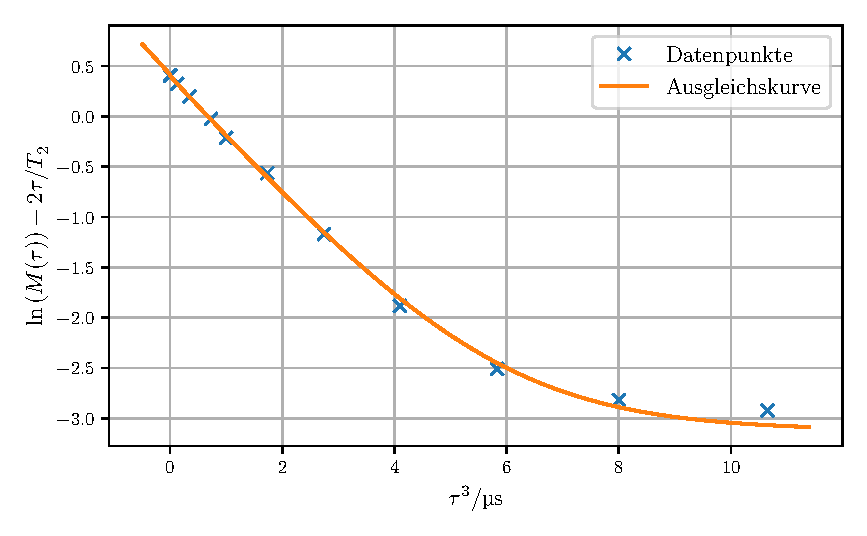
\includegraphics[width=\textwidth]{plots/echo.pdf}
    \caption{Die Daten wurden in einem linearen Zusammenhang aufgetragen und der Fit an die Daten ist auch dargestellt.}
    \label{abb:echo}
\end{figure}

Daraus wurde der Koeffizient $T_D$ und die beiden Amplitudenfaktoren $U_0$ und $U_1$ zu 
\begin{align*}
T_D &= \SI{1.69(4)e-6}{\per\second\tothe{3}} \\
M_0 &= \SI{1.47(1)}{\volt} \\
M_1 &= \SI{33.21(1264)}{\milli\volt} \\
\end{align*}
bestimmt.

Damit ergibt sich die Diffusionskonstante zu $D = \SI{1.882(33)e-9}{\meter\squared\per\second}$.
